\section*{Výsledky měření}

Pokud není uvedeno jinak, uvedené odchylky jsou standardní a odchylku nepřímo měřených veličin určujeme metodou přenosu chyby.
Používáme zápis $x=\SI{10(1)}{\cm}$, kde číslo v závorce vyjadřuje odchylku v řádu poslední uvedené číslice, tedy $x=\SI[separate-uncertainty=true]{10(1)}{\cm}$.


Pokus probíhal při normálním tlaku a pokojové teplotě ($t\approx\SI{22}{\degreeCelsius}$).

Měření jsme provedli se dvěma kruhovými cívkami, které budeme důsledně nazývat větší ($d=2r=\SI{40.5(5)}{\cm}$) a menší ($d=\SI{20.0(2)}{\cm}$).
Obě cívky měly 10 závitů a umožňovaly zapojení, ve kterém tekl proud jen 5 závity.
Měřili jsme tyčový magnet označený jako MAGNET2.

Na magnet jsme připevnili malé zrcadlo a zamířili jsme na něj laserový paprsek.
Do vzdálenosti $L=\SI{1.14(1)}{\m}$ od magnetu jsme umístili stínítko tak, aby na něj v rovnovážné poloze s nulovým proudem cívkou paprsek dopadal kolmo.

Pro obě cívky jsme měnili proud v rozmezí 0--\SI{4}{\ampere} a měřili výchylku místa dopadu laseru na stínítko. Proud jsme měřili vnějším ampérmetrem.
Pokud se vychýlil o $\Delta l$, úhel otočení magnetu určíme jako
\begin{equation}
\alpha = \frac{1}{2} \arctan \frac{\Delta l}{L} \,.
\end{equation}

Přímo hodnoty $\Delta l$ neuvádíme, naměřené úhly jsou uvedeny v tabulce \ref{tab:tabmain} a zaneseny do grafu \ref{graf:grafmain}


\begin{tabulka}[htbp]
\centering
\begin{tabular}{c|c|c|c|c}

 & \multicolumn{2}{c|}{menší cívka} & \multicolumn{2}{c}{větší cívka} \\
  & \multicolumn{2}{c|}{$r = \SI{10(1)}{\cm} $} & \multicolumn{2}{c}{$r= \SI{20.3(3)}{\cm} $} \\
  
  & $N=5$ & $N=10$ & $N=5$ & $N=10$ \\ \hline
  
$I$ (\si{\ampere}) & $\alpha$(\si{\degree}) & $\alpha$(\si{\degree}) & $\alpha$(\si{\degree}) & $\alpha$(\si{\degree}) \\
\hline

\num{0.5} & \num{0.40} & \num{0.80} & \num{0.23} & \num{0.45} \\
\num{1.0} & \num{0.80} & \num{1.63} & \num{0.43} & \num{0.85} \\
\num{1.5} & --- & \num{2.43} & --- & --- \\
\num{2.0} & \num{1.63} & \num{3.23} & \num{0.83} & \num{1.68} \\
\num{2.5} & --- & \num{4.04} & --- & --- \\
\num{3.0} & \num{2.43} & \num{4.83} & \num{1.26} & \num{2.48} \\
\num{3.5} & --- & \num{5.61} & --- & --- \\
\num{4.0} & \num{3.23} & \num{6.38} & \num{1.68} & \num{3.30} \\

\end{tabular}
\caption{Naměřená závislost úhlu otočení magnetu na volbě cívky a proudu jí protékajícím}
\label{tab:tabmain}
\end{tabulka}

\begin{graph}[htbp] 
\centering
% GNUPLOT: LaTeX picture with Postscript
\begingroup
  \makeatletter
  \providecommand\color[2][]{%
    \GenericError{(gnuplot) \space\space\space\@spaces}{%
      Package color not loaded in conjunction with
      terminal option `colourtext'%
    }{See the gnuplot documentation for explanation.%
    }{Either use 'blacktext' in gnuplot or load the package
      color.sty in LaTeX.}%
    \renewcommand\color[2][]{}%
  }%
  \providecommand\includegraphics[2][]{%
    \GenericError{(gnuplot) \space\space\space\@spaces}{%
      Package graphicx or graphics not loaded%
    }{See the gnuplot documentation for explanation.%
    }{The gnuplot epslatex terminal needs graphicx.sty or graphics.sty.}%
    \renewcommand\includegraphics[2][]{}%
  }%
  \providecommand\rotatebox[2]{#2}%
  \@ifundefined{ifGPcolor}{%
    \newif\ifGPcolor
    \GPcolorfalse
  }{}%
  \@ifundefined{ifGPblacktext}{%
    \newif\ifGPblacktext
    \GPblacktexttrue
  }{}%
  % define a \g@addto@macro without @ in the name:
  \let\gplgaddtomacro\g@addto@macro
  % define empty templates for all commands taking text:
  \gdef\gplbacktext{}%
  \gdef\gplfronttext{}%
  \makeatother
  \ifGPblacktext
    % no textcolor at all
    \def\colorrgb#1{}%
    \def\colorgray#1{}%
  \else
    % gray or color?
    \ifGPcolor
      \def\colorrgb#1{\color[rgb]{#1}}%
      \def\colorgray#1{\color[gray]{#1}}%
      \expandafter\def\csname LTw\endcsname{\color{white}}%
      \expandafter\def\csname LTb\endcsname{\color{black}}%
      \expandafter\def\csname LTa\endcsname{\color{black}}%
      \expandafter\def\csname LT0\endcsname{\color[rgb]{1,0,0}}%
      \expandafter\def\csname LT1\endcsname{\color[rgb]{0,1,0}}%
      \expandafter\def\csname LT2\endcsname{\color[rgb]{0,0,1}}%
      \expandafter\def\csname LT3\endcsname{\color[rgb]{1,0,1}}%
      \expandafter\def\csname LT4\endcsname{\color[rgb]{0,1,1}}%
      \expandafter\def\csname LT5\endcsname{\color[rgb]{1,1,0}}%
      \expandafter\def\csname LT6\endcsname{\color[rgb]{0,0,0}}%
      \expandafter\def\csname LT7\endcsname{\color[rgb]{1,0.3,0}}%
      \expandafter\def\csname LT8\endcsname{\color[rgb]{0.5,0.5,0.5}}%
    \else
      % gray
      \def\colorrgb#1{\color{black}}%
      \def\colorgray#1{\color[gray]{#1}}%
      \expandafter\def\csname LTw\endcsname{\color{white}}%
      \expandafter\def\csname LTb\endcsname{\color{black}}%
      \expandafter\def\csname LTa\endcsname{\color{black}}%
      \expandafter\def\csname LT0\endcsname{\color{black}}%
      \expandafter\def\csname LT1\endcsname{\color{black}}%
      \expandafter\def\csname LT2\endcsname{\color{black}}%
      \expandafter\def\csname LT3\endcsname{\color{black}}%
      \expandafter\def\csname LT4\endcsname{\color{black}}%
      \expandafter\def\csname LT5\endcsname{\color{black}}%
      \expandafter\def\csname LT6\endcsname{\color{black}}%
      \expandafter\def\csname LT7\endcsname{\color{black}}%
      \expandafter\def\csname LT8\endcsname{\color{black}}%
    \fi
  \fi
  \setlength{\unitlength}{0.0500bp}%
  \begin{picture}(10204.00,6802.00)%
    \gplgaddtomacro\gplbacktext{%
      \csname LTb\endcsname%
      \put(814,704){\makebox(0,0)[r]{\strut{} 20}}%
      \csname LTb\endcsname%
      \put(814,1676){\makebox(0,0)[r]{\strut{} 30}}%
      \csname LTb\endcsname%
      \put(814,2648){\makebox(0,0)[r]{\strut{} 40}}%
      \csname LTb\endcsname%
      \put(814,3621){\makebox(0,0)[r]{\strut{} 50}}%
      \csname LTb\endcsname%
      \put(814,4593){\makebox(0,0)[r]{\strut{} 60}}%
      \csname LTb\endcsname%
      \put(814,5565){\makebox(0,0)[r]{\strut{} 70}}%
      \csname LTb\endcsname%
      \put(814,6537){\makebox(0,0)[r]{\strut{} 80}}%
      \csname LTb\endcsname%
      \put(946,484){\makebox(0,0){\strut{} 0}}%
      \csname LTb\endcsname%
      \put(2718,484){\makebox(0,0){\strut{} 20}}%
      \csname LTb\endcsname%
      \put(4490,484){\makebox(0,0){\strut{} 40}}%
      \csname LTb\endcsname%
      \put(6263,484){\makebox(0,0){\strut{} 60}}%
      \csname LTb\endcsname%
      \put(8035,484){\makebox(0,0){\strut{} 80}}%
      \csname LTb\endcsname%
      \put(9807,484){\makebox(0,0){\strut{} 100}}%
      \put(176,3620){\rotatebox{-270}{\makebox(0,0){\strut{}Povrchové napětí (\num{e-3}\,\si{\newton\per\metre})}}}%
      \put(5376,154){\makebox(0,0){\strut{}Koncentrace lihu (\si{\percent})}}%
    }%
    \gplgaddtomacro\gplfronttext{%
    }%
    \gplbacktext
    \put(0,0){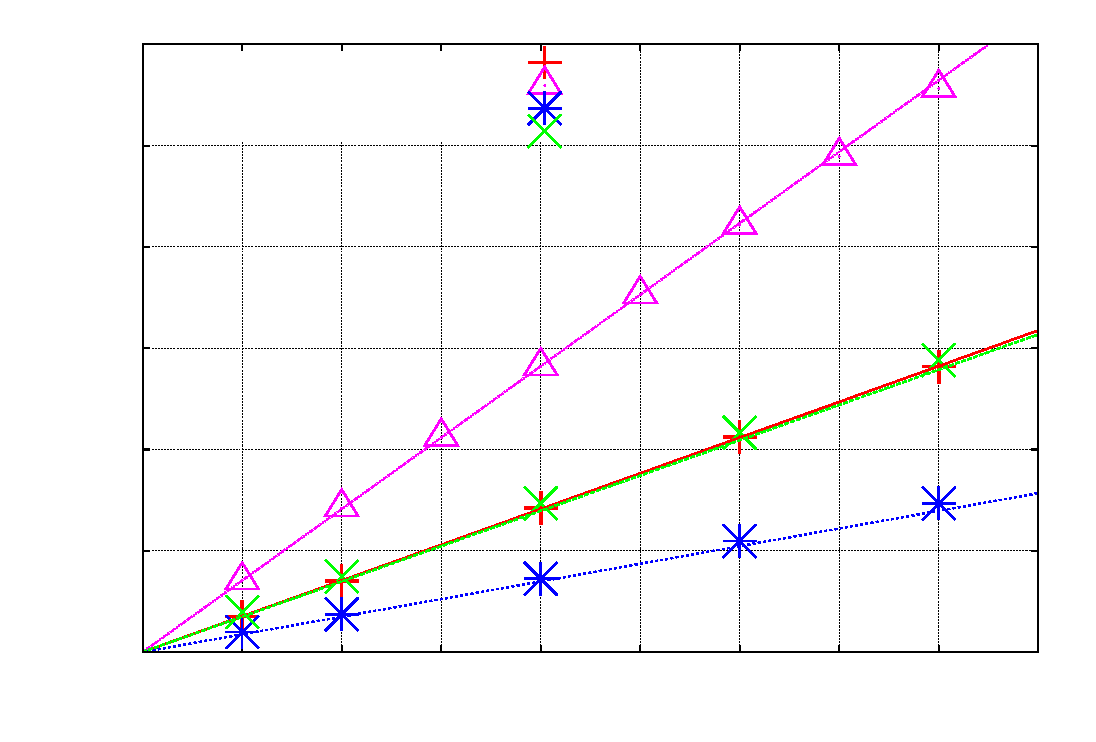
\includegraphics{graf}}%
    \gplfronttext
  \end{picture}%
\endgroup

\caption{Naměřená závislost úhlu otočení magnetu na volbě cívky a proudu jí protékající, teoretická závislost \eqref{eq:vzorecalfa} s nafitovaným magnetickým momentem $p$}
\label{graf:grafmain}
\end{graph}


Pro změření direkčního momentu vlákna jsme na něj zavěsili mosaznou tyč o délce $l_t=\SI{24.0(1)}{\cm}$, hmotnosti $m_t=\SI{56.6}{\g}$ a průměru $d_t=\SI{6}{\mm}$.
Moment setrvačnosti takové tyče vzhledem k ose procházející průměrem v~jejím středu je podle \cite{momentset}
\begin{equation} \label{eq:momentsetrvacnosti}
J=m(d_t^2+\frac{1}{12} l_t^2)= \SI{2.74e-4}{\kg\m\squared} \,.
\end{equation}
Změřili jsme dobu 20 kmitů \SI{80.5}{\s}, tedy perioda $T=\SI{4.03}{\s}$.
Direkční moment vlákna jsme určili podle \eqref{eq:periodadirekcnimoment} $D=\num{6.6(2)}\cdot \SI{e-4}{\newton\metre\per\radian}$. Odchylku jsme odhadli na \SI{3}{\percent}.

Naměřenou závislost \eqref{eq:vzorecalfa} jsme nafitovali Coulombovým magnetickým momentem $p = \num{3.8(2)} \cdot \SI{e-7}{\weber \meter}$.
Vzhledem k nepřesnostem při měření jsme odchylku odhadli na \SI{5}{\percent}.
Ampérův magnetický moment vypočítáme podle \eqref{eq:amper} jako $m = \SI{0.30(2)}{\ampere\metre\squared}$.
Teoretickou závislost \eqref{eq:vzorecalfa} jsme zanesli do grafu \ref{graf:grafmain} pro porovnání s naměřenými veličinami.